\documentclass[12pt,twoside]{article}
\usepackage{jmlda}
\usepackage{url}
\usepackage{hyperref}

\makeatletter
\bibliographystyle{unsrt}
\renewcommand{\@biblabel}[1]{#1.}
\makeatother

%\NOREVIEWERNOTES
\title
    [Аппроксимация фазовой траектории] 
    % Краткое название; не нужно, если полное название влезает в~колонтитул
    {Аппроксимация фазовых траекторий квазипериодических временных сигналов с помощью сферических гармоник}
\author
    {Тихонов~Д.\,М., Стрижов~В.\,В.} % основной список авторов, выводимый в оглавление
    %\thanks
    %{Работа выполнена при финансовой поддержке РФФИ, проект \No\,00-00-00000.}
%\email
   % {author@site.ru}
%\organization
   % {$^1$Организация; $^2$Организация}
%\thanks
%	{ }
\abstract
{\textbf{Аннотация}: В этой работе обсуждается проблема построения модели для фиксированного класса квазипериодических сигналов наименьшей структурной сложности.
Структурная сложность - это число настраиваемых параметров модели.
Для перехода в фазовое пространство временной ряд векторизуется с помощью метода задержек.
Для понижения сложности модели в фазовом пространстве выбирается подпространство.
Вводится критерий выбора оптимальной размерности подпространства.
Фазовая траектория в полученном подпространстве аппроксимируется с помощью сферических гармоник.
Радиус восстанавливается с помощью линейной модели.
Вычислительный эксперимент проведен на измерениях акселерометра мобильного устройства с $4$ классами движений человека.

\bigskip
\textbf{Ключевые слова}: \emph {временные ряды, аппроксимация, фазовое пространство, сферические гармоники}.}

    

\newcommand{\nsymbol}[2]{\medskip\hangindent=\parindent\hangafter=1\noindent $#1$ --- #2\par}
\newcommand{\nsymbolp}[3]{\nsymbol{#1}{#2 \dotfill\pageref{#3}}}

\newcommand{\hookuparrow}{\mathrel{\rotatebox[origin=t]{270}{$\hookleftarrow$}}}
\newcommand{\hookdownarrow}{\mathrel{\rotatebox[origin=t]{90}{$\hookleftarrow$}}}
\begin{document}
\maketitle

\section{Введение}
Работа посвящена аппроксимации квазипериодических временных рядов.
Примерами таких рядов являются показатели акселерометра и гироскопа во время повторяющейся физической активности, электрокардиограмма.

Различные методы аппроксимации имеют свои особенности, ограничениями и недостатками.
Существуют решения проблемы на плоскости, то есть только с данными размерности два ~\cite{Fitzgibbon1999, Ahn1998}.
Ограничение размерности сужает области применения подобных решений.
Предлагаются методы~\cite{Fitzgibbon1999, Rosin1995}, основанные на минимизации критериев алгебраического расстояния.
Критерии не имеют геометрической интерпретации, поскольку они не связаны в явном виде с евклидовыми расстояниями.
Поэтому такие методы могут некорректно сохранять информацию о положении точек.
Нейросетевые модели ~\cite{Andras2017, Cheridito2021} являются структурно сложными с большим числом настраиваемых параметров.
Это приводит к неустойчивости и сложной интерпретируемости моделей.
В работе ~\cite{Calafiore2002} для аппроксимации используются  сферы и эллипсоиды.
Такой подход устойчиво аппроксимирует, но теряет информацию о локальной геометрической структуре.
%алгоритмы основанные на дисперсионном анализе (ANOVA) %~\cite{potts2021interpretable}.
	
В этой работе предлагается модель аппроксимации временных рядов.
Для этого производится переход в пространство фазовых траекторий или траекторное пространстве .
Переход осуществляется методом задержек~\cite{LAI19961}.
Метод задержек используется при анализе нестационарных временных рядов.
Например, в методе сингулярного спектрального анализа~\cite{Golyandina2002} разложения на компоненты и прогноз основаны на траекторной матрице.
Она позволяет перейти от скалярного временного ряда к многомерному представлению.
Метод задержек так же получили широкое распространение в анализе нелинейных динамических систем~\cite{Takens1981, LAI19961}.

Избыточная размерность траекторного пространства ~\cite{Golyandina2002, Motrenko2015,Usmanova2020} приводит к неустойчивости исследуемых моделей и избыточно сложному описанию временного ряда.
Для понижения размерности фазового пространства предлагается использовать  метод главных компонент~\cite{Ezukwoke2019, Scholkopf1998}. Рассматривается

В выбранном пространстве пониженной размерности фазовая траектория проецируется на $p$-мерную единичную сферу.
Полученную на поверхности сферы функцию предлагается представить в виде ряда разложенного по сферическим гармоникам.
Радиус восстанавливается линейной моделью по имеющимся значениям углов.

\begin{figure}[h]
\centering
  \subfloat[$s(t) = 2cos(2\pi\nu_1t + \varphi_1) + cos(2\pi\nu_2t + \varphi_2) + \varepsilon$]
  {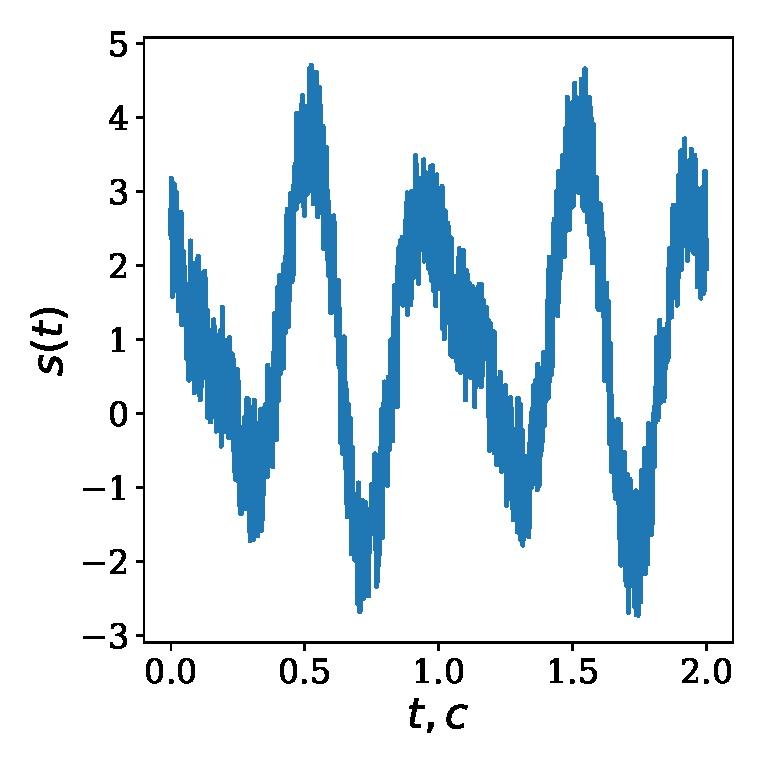
\includegraphics[width=0.25\textwidth]{figs/synthetic_example.eps}}
  \subfloat[Фазовая траектория (PCA)]
  {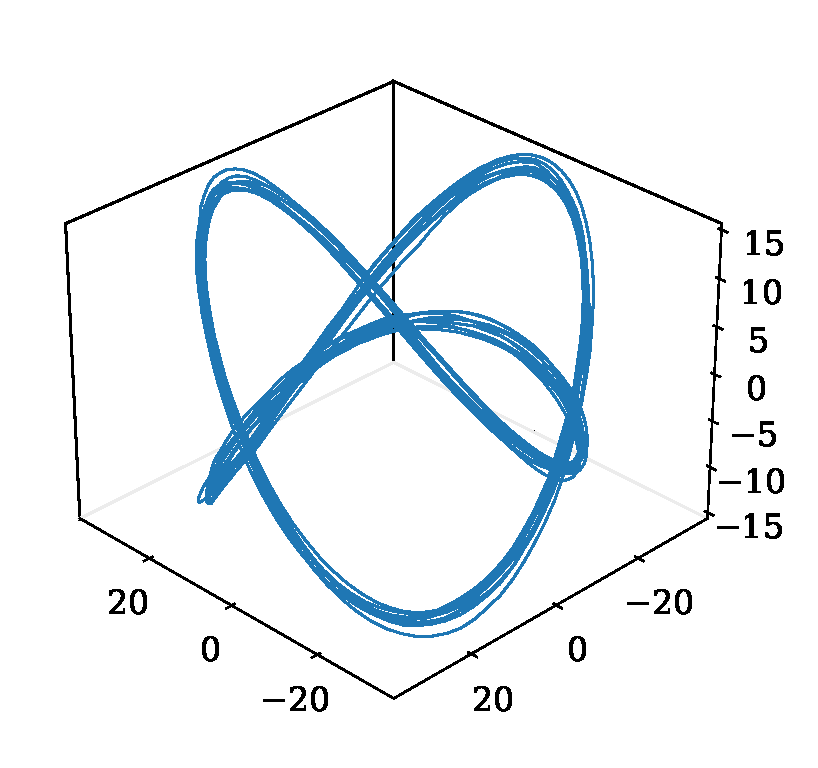
\includegraphics[width=0.3\textwidth]{figs/synthetic_trajectory.eps}}\\
\caption{Временной ряд с параметрами $\nu_1 = 2\;[\frac{1}{c}], \varphi_1 = 0,\nu_2 = 3\;[\frac{1}{c}],\varphi_2 = \frac{3\pi}{4}$ и его фазовая траектория. }
\label{fg:initial_traj}
\end{figure}

На рис.~\ref{fg:initial_traj} показан изначальный временной ряд и его фазовая траектория в пространство размерности 3.
Фазовая траектория получена с помощью метода анализ главных компонент над матрицей задержек.

%%%%%%%%%%%%%%%%%%%%%%%%%%%%%%%%%%%%%%%%%%%%%%%%%%%%%%%%%%%%%%%%%%%%%%%%%%%%%
\section{Постановка задачи}
По имеющемуся временному ряду $\mathbf{s}=[s_1,...,s_N]^{\mathsf{T}}$ с помощью метода задержек строится траекторная матрица

\begin{equation}
\mathbf{H}_{s}^{n} = 
\begin{bmatrix} 
	s_{1} & s_{2} & \ldots &s_{n-1} &s_{n}\\
	s_{2} & s_{3} & \ldots &s_{n} &s_{n+1}\\
	\vdots& \vdots & \ddots & \vdots & \vdots\\
	s_{N-n+1} & s_{N-n+2} &\ldots&s_{N-1} &s_{N}\\
\end{bmatrix},
\label{eq:hankel_matrix}
\end{equation}
где $N$-длина временного ряда, $n$-ширина окна, не меньшая, чем предполагаемый период.

Вводится обозначение $t$-ой строк траекторной матрицы $\mathbf{H}_{s}$. Тогда матрица $\mathbf{H}_{s}$ преобразуется к:	
\begin{equation}
	\mathbf{H}_{s}^{n} = 
	\begin{bmatrix} 
      	\mathbf{s}_{1}\\
      	\mathbf{s}_{2}\\
      	\vdots\\
      	\mathbf{s}_{m}\\
   \end{bmatrix},
   \quad
   \mathbf{s}_t=[s_{t},s_{t+1},\ldots,s_{t+n-1}],
   \quad
   m = N-n+1,
\label{eq:hankel_matrix_2}
\end{equation}
\vspace{\baselineskip}
где векторы $\mathbf{s_{t}} \in \mathbb{H}_{s} \subseteq \mathbb{R}^{n}$ и образуют фазовую траекторию ряда $\mathbf{s}$.

Предполагается, что размерность траекторного пространства $\mathbb{H}_{s}^{n}$ избыточна.
Поэтому предлагается исследовать некоторые его проекции на траекторное подпространство $\mathbb{H}_{p}^{n}$.
Однако заранее неизвестно, в каком пространстве необходимо уменьшать размерность, поэтому задача приобретает следующий вид:

\begin{equation}
	t
	\mapsto
	\mathbf{x}
	\mapsto
	\mathbb{H}_{s}^{n}
	\xrightarrow{}
	\mathbb{H}_{x}^{p}
	\xrightarrow{}
	\mathbb{S}_z^{p}
	\hookrightarrow
	[0,2\pi]
	\xrightarrow{f}
	r
\label{eq:goal}
\end{equation}

\vspace{\baselineskip}

\begin{Def}
Параметрическая аппроксимирующая модель временного ряда  $\mathbf{s}$  - это такое отображение $g$, что
\begin{equation}
	g: \mathbb{R}^{q} \times \mathbf{S} \xrightarrow{} \mathbf{S}.
\label{eq:param_model}
\end{equation}
\end{Def}

Предполагается, что аппроксимирующая модель строится в пространстве меньшей размерности $p$, в котором выбранное отображение
\begin{equation}
h: \mathbf{H}_{s}^{n} \xrightarrow{} \mathbf{S}_x^{p},
\label{eq:tomindimmodel}
\end{equation}

где $p \ll n$, сохраняет геометрическую структуру множество точек $\mathbf{H}_{s}^{n}$. 
\begin{Def}
Структурная сложность - это число параметров $q$ модели, позволяющих строить адекватную аппроксимацию.
\end{Def}

%%%%%%%%%%%%%%%%%%%%%%%%%%%%%%%%%%%%%%%%%%%%%%%%%%%%%%%%%%%%%%%%%%%%%%%%%%%%%
\section{Аппроксимация сферическими гармониками}

Предполагается, что структура модели проще в сферических координатах.
Переход к сферическому представлению временного ряда состоит из двух этапов.

Первый этап - переход в подпространство $\mathbb{H}_{x}^{n} \xrightarrow{} \mathbb{H}_{x}^{p}$ по алгоритму PCA при $p \ll n $:
\[
\mathbf{H}_{x}^{p} = \mathbf{H}_{s}^{n}\mathbf{U} =
\begin{bmatrix} 
  	\mathbf{x}_{1}\\
  	\mathbf{x}_{2}\\
  	\vdots\\
  	\mathbf{x}_{m}\\
\end{bmatrix},
\quad
\mathbf{x}_{t} \in \mathbb{R}^{p},
\quad
t \in [1,m]
\]
где $\mathbf{U}$ --- матрица преобразования алгоритма PCA с количеством компонент равным $p$, соответствующим наибольшим собственным значениям.

Второй этап - переход в сферические координаты в полученном подпространстве $\mathbb{H}_{x}^{p}$.
Строится отображение из декартовых координат в сферические $\mathbb{H}_{x}^{p} \xrightarrow{} \mathbb{S}_{z}^{p}$:
\[
    \phi: \mathbf{x} \xrightarrow{} \mathbf{z} = [r,\alpha_{p-1},\dots,\alpha_1],
    \quad
    \mathbf{a} = [\alpha_{p-1},\dots,\alpha_1]
\]

Для выбора оптимальной размерности подпространства вводится критерий.
\begin{Def}
Оптимальная размерность $\hat{p}$- это такая размерность , что любые 2 точки фазовой траектории с существенно разным моментам времени внутри одного периода не находятся в окрестности друг друга.
Точки фазовой траектории представлены сферических координатах на поверхности единичной сферы.
\end{Def}

\begin{equation}           
    \hat{p} = \argmin_{p \in \{1, \dots, n \}}
    \sum_{t=1}^m \mathbf{1}_A(\mathbf{a}_t),
    \quad
    A = \{\mathbf{z}_i|
        \rho(\mathbf{a}_{t_i},\mathbf{a}_{t_j}) \leq \epsilon,
        \quad
        \frac{T}{4} \leq |t_i - t_j| \leq \frac{3T}{4},
        \quad
        i,j \in [1,m],
        \}
\label{eq:intersection_criterion} 
\end{equation}
где $T$ - предполагаемый период ряда $\mathbf{s}$, $\rho$ - метрика определенная в пространстве углов.

Предлагается выбрать $\rho(\cdot)$ в виде:
\[
    \rho(\mathbf{a},\mathbf{a}') = \frac{1 - cos(\langle \mathbf{a},\mathbf{a}' \rangle)}{2},
    \quad
	\mathbf{a} = [\alpha_{1},\dots, \alpha_{p-1}],
	\quad
	\alpha_t \in [0,2\pi)
	\quad
	t \in [1,p-1]
\]

В пространства размерности, выбранной таким образом \ref{eq:intersection_criterion}, строится взаимно однозначное соответствие между временем и отрезку фазовой траектории.
То есть определенной области пространства соответствует строго одна область временного промежутка внутри периода. 

Аппроксимация модель включает в себя две составляющие.
Первая  часть $f_{sp}(\cdot)$ аппроксимирует функцию полученную проекцией на сферу.
То есть из множества всевозможных углов $\hat{A} = [0,\pi)\times[0,2\pi)\times \dots \times [0,2\pi)$ выделяет $A \subseteq \hat{A}$, на которых определена фазовая траектория.
\begin{equation}
    f_{sp}: \mathbb{R}^{|\mathbf{{w}}_{sp}|} \times \hat{A}
    \mapsto
    A
\label{eq:f_sp}
\end{equation}

В качестве базисных функций на поверхности $(p-1)$-мерной сферы выберем сферические гармоники:

\begin{equation}
	Y_{l_{p-1},...,l_1}(\alpha_{p-1},\dots,\alpha_1) = 
	\left[
	    \prod\limits_{k = 2}^{p-1}
	    {_k}{\overline{P}}_{l_k}^{l_{p-1}}(\alpha_k)
	\right]
	    \frac{1}{\sqrt{2\pi}}
	    \exp{(i l_1 \alpha_1)},
\label{eq:YlN}
\end{equation}
где $l_{p-1},...,l_1$ - индексы удовлетворяющие
\[l_{p-1} \geq l_{p-2} \geq \dots \geq l_2 \geq|l_1|.\]

За функцию $_k\mathbf{\overline{P}}_{L}^{l}(\alpha_k)$ обозначается  
\[
   _k\mathbf{\overline{P}}_{l}^{L}(\alpha) =
   {_k}c^l_L \cdot (\sin \alpha)^{\frac{-(k-2)}{2}}
   \mathbf{P}^{-(l+\frac{(k-2)}{2})}_{L+\frac{(n-2)}{2}}(\cos \alpha)
\]
где $\mathbf{P}_{\mu}^{-\eta}(x)$ - соответствующие полиномы Лежандра, ${_k}c^l_L$ - нормировочный коэффициент
\[
    {_k}c^l_L = 
        \left[
	        \frac{2L+k-1}{2}
	        \frac{(L+l+k-2)!}{(L-l)!}
	    \right]^{\frac{1}{2}}.
\]

В частности при $p = 3$ (\ref{eq:YlN}) приобретает вид
\begin{equation}
	Y_{m,l}(\alpha_1,\alpha_2) = \sqrt{ \frac{(2l+1)}{4\pi} \frac{(l-m)!}{(l+m)!} } P_l^m(cos\alpha_2)e^{im\alpha_1}.
\label{eq:Yml}
\end{equation}

В классическом виде сферические гармониками определены в комплексном пространстве. В исследуем случае нет необходимости в реальной и комплексной части одновременно. Для простоты программирования и поскольку многие из желаемых свойств присутствуют, используется только либо действительная, либо комплексная часть. Это рассчитывается следующим образом:

\begin{equation}
	RIY_{l_{p-1},...,l_1}(\alpha_{p-1},\dots,\alpha_1) = \begin{cases}
	\text{Re}(Y_{l_{p-1},...,l_1}(\alpha_{p-1},\dots,\alpha_1)), & \mbox{если } l_1 \geq 0\\
    \text{Im}(Y_{l_{p-1},...,l_1}(\alpha_{p-1},\dots,\alpha_1)), & \mbox{иначе}.
    \end{cases}
\label{eq:RTY}
\end{equation}

\vspace{\baselineskip}

Тогда аппроксимирующая функция представима в виде
\begin{equation}
	f_{sh}(\mathbf{w}_{sp},\mathbf{a}) = \sum_{l_{p-1} = 0}^{N_{approx}}
	                                \sum_{l_{p-2} = 0}^{l_{p-1}}
	                                \dots 
	                                \sum_{l_1 = -l_2}^{l_2}  
	                                w_{l_{p-1},...,l_1} RIY_{l_{p-1},...,l_1}(\alpha_{p-1},\dots,\alpha_1)
\label{eq:f_ph_3d}
\end{equation}
где $N_{approx}$ - порядок приближения. 
\vspace{\baselineskip}

\begin{figure}[h]
\centering
\includegraphics[width=0.3\textwidth]{figs/sp_mesh.eps}
\caption{Сетка на поверхности сферы}
\label{fg:sp_mesh}
\end{figure}

Для получения упрощения задачи множество $\hat{A}$ дискретизируется на поверхности сферы. Пример дискретизации в трехмерном случае показан показан на рисунке~(\ref{fg:sp_mesh}).
Теперь $\hat{A} = \{\hat{\mathbf{a}}_i,...,\hat{\mathbf{a}}_d\}$, где $d$ - количество точке или мелкость разбиения.
По дискретному набору точек производится построение функции дискретной функции $F(\hat{\mathbf{a}})$:

\begin{equation}
    F(\mathbf{\hat{\mathbf{a}}}) =
    \begin{cases}
	1, & \mbox{если } \exists \mathbf{a} \in O_{\delta}(\hat{\mathbf{a}}),
	\;\mathbf{a} \in A,\;\mathbf{\hat{a}} \in \hat{A}\\
    0, & \mbox{иначе}.
    \end{cases}
\label{eq:f_real}
\end{equation}



% Тогда аппроксимирующая функция представима в виде
% \begin{equation}
% 	f_{ph}(\mathbf{w},\alpha_1,\alpha_2) = \sum_{n,m \in N,M} w_{n,m}Y_l^m(\alpha_1,\alpha_2)
% \label{eq:f_ph_3d}
% \end{equation}
% \vspace{\baselineskip}

% Функцию потерь представляется в виде
% \begin{equation}
% \textrm{Loss} =  \sum_{n,m \in N,M} \hat{f}_{ph}(\mathbf{w},\alpha_1,\alpha_2) - f_{real}(\alpha_{1},\alpha_2)
% \label{eq:L_3d}
% \end{equation}

Тогда задачу аппроксимации можно представить в виде 

\begin{equation}
\begin{pmatrix} 
	RIY_{l_{p-1},...,l_1}(\hat{\mathbf{a}}_1) & \ldots &RIY_{0,...,0}(\hat{\mathbf{a}}_1)\\
	\vdots& \ddots & \vdots\\
	RIY_{l_{p-1},...,l_1}(\hat{\mathbf{a}}_d) & \ldots &RIY_{0,...,0}(\hat{\mathbf{a}}_d)\\
\end{pmatrix}
\begin{pmatrix} 
	w_{l_{p-1},...,l_1}\\
	\vdots\\
	w_{0,...,0}\\
\end{pmatrix}
=
\begin{pmatrix} 
	F(\hat{\mathbf{a}}_1)\\
	\vdots\\
	F(\hat{\mathbf{a}}_d)\\
\end{pmatrix}
\label{eq:sp_app_matrix}
\end{equation}
или в более короткой записи:
\begin{equation}
\mathbf{X}\mathbf{w}_{sp} =\mathbf{F}
\label{eq:sp_app_matrix_short}
\end{equation}

Такая постановка позволяет свести решения к МНК, что существенно ускоряет процесс обучения из-за существования аналитического решения.
Однако, в силу экспоненциального роста количества сферических гармоник в случае повышения размерности пространства, необходимо вводить регуляризаторы. 

\begin{equation}
    \mathbf{\hat{w}}_{sp} = \argmin_{\mathbf{w}_{sp}}
    \|\mathbf{X}\mathbf{w}_{sp} - \mathbf{F}\|^2 + \lambda\|\mathbf{w}_{sp}\|^2
\label{eq:arg_l2}
\end{equation}
Ее решение представимо аналитически в виде:
\begin{equation}
    \mathbf{\hat{w}}_{sp} = (\lambda \mathbf{I} - \mathbf{X}^T\mathbf{X})^{-1}\mathbf{X}^T\mathbf{F}
\label{eq:arg_l2_solution}
\end{equation}
Вторая часть - это регрессионная модель $f_r(\cdot)$, восстанавливает по переменным $\mathbf{a} \in \hat{A}$ радиус $r$.
\begin{equation}
    f_r: \mathbf{a}
    \mapsto
    \hat{r}
\label{eq:arg_l}
\end{equation}
\[
\hat{r} = f_r(\mathbf{\hat{w}_r},\alpha_{1},\dots, \alpha_{p-1}) = \mathbf{\hat{w}_r}^T\,\mathbf{a}
\]
\[
\mathbf{\hat{w}_r} = \argmin_{\mathbf{w_r}}(r - \mathbf{\hat{w}_r}^T\,\mathbf{a})^2
\]

Комбинация моделей  $ g = g(f_r(\cdot),f_{sp}(\cdot))$ позволяет с помощью подбираемых параметров $\mathbf{\hat{w}_r}$ и $\mathbf{\hat{w}_{sp}}$ полностью параметризовать фазовою траекторию вместе с областью дисперсии.


\section{Эксперимент}
\paragraph{Аппроксимация сферическими гармониками}
\begin{table}
    \centering
        \begin{tabular}{p{0.5cm}p{3cm}p{4cm}p{4cm}}
              & Временной ряд
              & Фазовая траектория в 3D
              & Аппроксимация гармониками
              \\
            \hline
            \rotatebox{90}{ \text{Велопрогулка} }
            & \includegraphics[scale=0.2]{./figs/bike_example.eps}
            & \includegraphics[scale=0.3]{./figs/bike_trajectory.eps}
            & \includegraphics[scale=0.25]{./figs/sph_harm_bike.eps}
            \\ 
            \hline
            
            \rotatebox{90}{ \text{Приседания} }
            & \includegraphics[scale=0.2]{./figs/squats_example.eps}
            & \includegraphics[scale=0.3]{./figs/squats_trajectory.eps}
            & \includegraphics[scale=0.25]{./figs/sph_harm_squats.eps} \\ 
            \hline
        \end{tabular}
    \caption{Таблица сравнений разных классов движений}
    \label{tbl:table_of_figures}
\end{table}


% \begin{figure}[h]
% \centering
% \includegraphics[width=0.5\textwidth]{figs/3D_sp_harm}
% \caption{Аппроксимация сферическими гармониками 3D. }
% \label{fg:3D_sp_harm}
% \end{figure}

\section{Заключение}
\newpage
\bibliography{lib}

\end{document}
